	\documentclass[12pt,a4paper]{report}
\usepackage[latin1]{inputenc}
\usepackage{amsmath}
\usepackage{amsfonts}
\usepackage{amssymb}
\usepackage{graphicx}
\usepackage{multicol}
\usepackage{float}

\title{Continuous Asessment: ECM1417}
\begin{document}
	\maketitle
	\newpage
	\section{Database}
	\paragraph{Schema:}
	The database has three tables, a users table, a stock information table and a stock entries table. These tables allow for logging of stock entries and ease of user management. The schema is as follows:
	\begin{multicols}{3}
	\subparagraph{Users:}
	\begin{itemize}
		\item UserID \\ INT \\ Primary key
		\item username \\ VARCHAR(20) \\ UNIQUE
		\item Name \\ VARCHAR(30)
		\item HashedPW \\ BINARY(60)
		\item Permissions \\ INT
	\end{itemize}
	\columnbreak
	\subparagraph{StockInfo:}
	\begin{itemize}
		\item StockID \\ INT \\ Primary key
		\item StockName \\ VARCHAR(255)
		\item StockPrice \\ INT
		\item CurrentQuantity \\ INT
		\item LastModified \\ TIMESTAMP
		\item LastModifiedBy \\ INT
		\item UserID \\ INT
		\item TimeCreated \\ TIMESTAMP
	\end{itemize}
	\columnbreak
	\subparagraph{StockEntries:}
	\begin{itemize}
		\item EntryID \\ INT \\ Primary key
		\item StockID \\ INT
		\item ChangeType \\ INT
		\item Amount \\ INT
		\item TimeCreated \\ TIMESTAMP
		\item CreatedBy \\ INT
	\end{itemize}
	\end{multicols}
	There are four relationships between the tables:
	\begin{itemize}
		\item Users.UserID $\leftarrow$ one to many $\rightarrow$ StockInfo.UserID.
		\item Users.UserID $\leftarrow$ one to many $\rightarrow$ StockInfo.LastModifiedBy.
		\item Users.UserID $\leftarrow$ one to many $\rightarrow$ StockEntries.CreatedBy.
		\item StockInfo.StockID $\leftarrow$ one to many $\rightarrow$ StockEntries.StockID.
	\end{itemize}
	\paragraph{Reasons}
	This method of storing the stock data is useful as it allows an admin to get a record of what has changed and manage users. A trigger on the StockInfo table updates the LastModified and LastModifiedBy columns with the values of the latest entry in StockEntries with the same StockID. The permissions column allows a user to be restricted in what they are allowed to do changing the pages they visit and blocking them from submitting some forms. There are two ways of changing the Stock, "change" and "set". They are intended for different purposes; a "change" stock is when a new shipment arrives or some stock is sold, the stock changes by some amount. A "set" stock an the other hand is intended for when something like a stock count is done, if there is same discrepancy between the current stock amount and the counted amount it can be resolved by simply setting the current stock count to one that was just found.
	\section{UI}
	\subsection{Index}
	\begin{figure}[!ht]
		\hspace*{-1in}
		\centering
		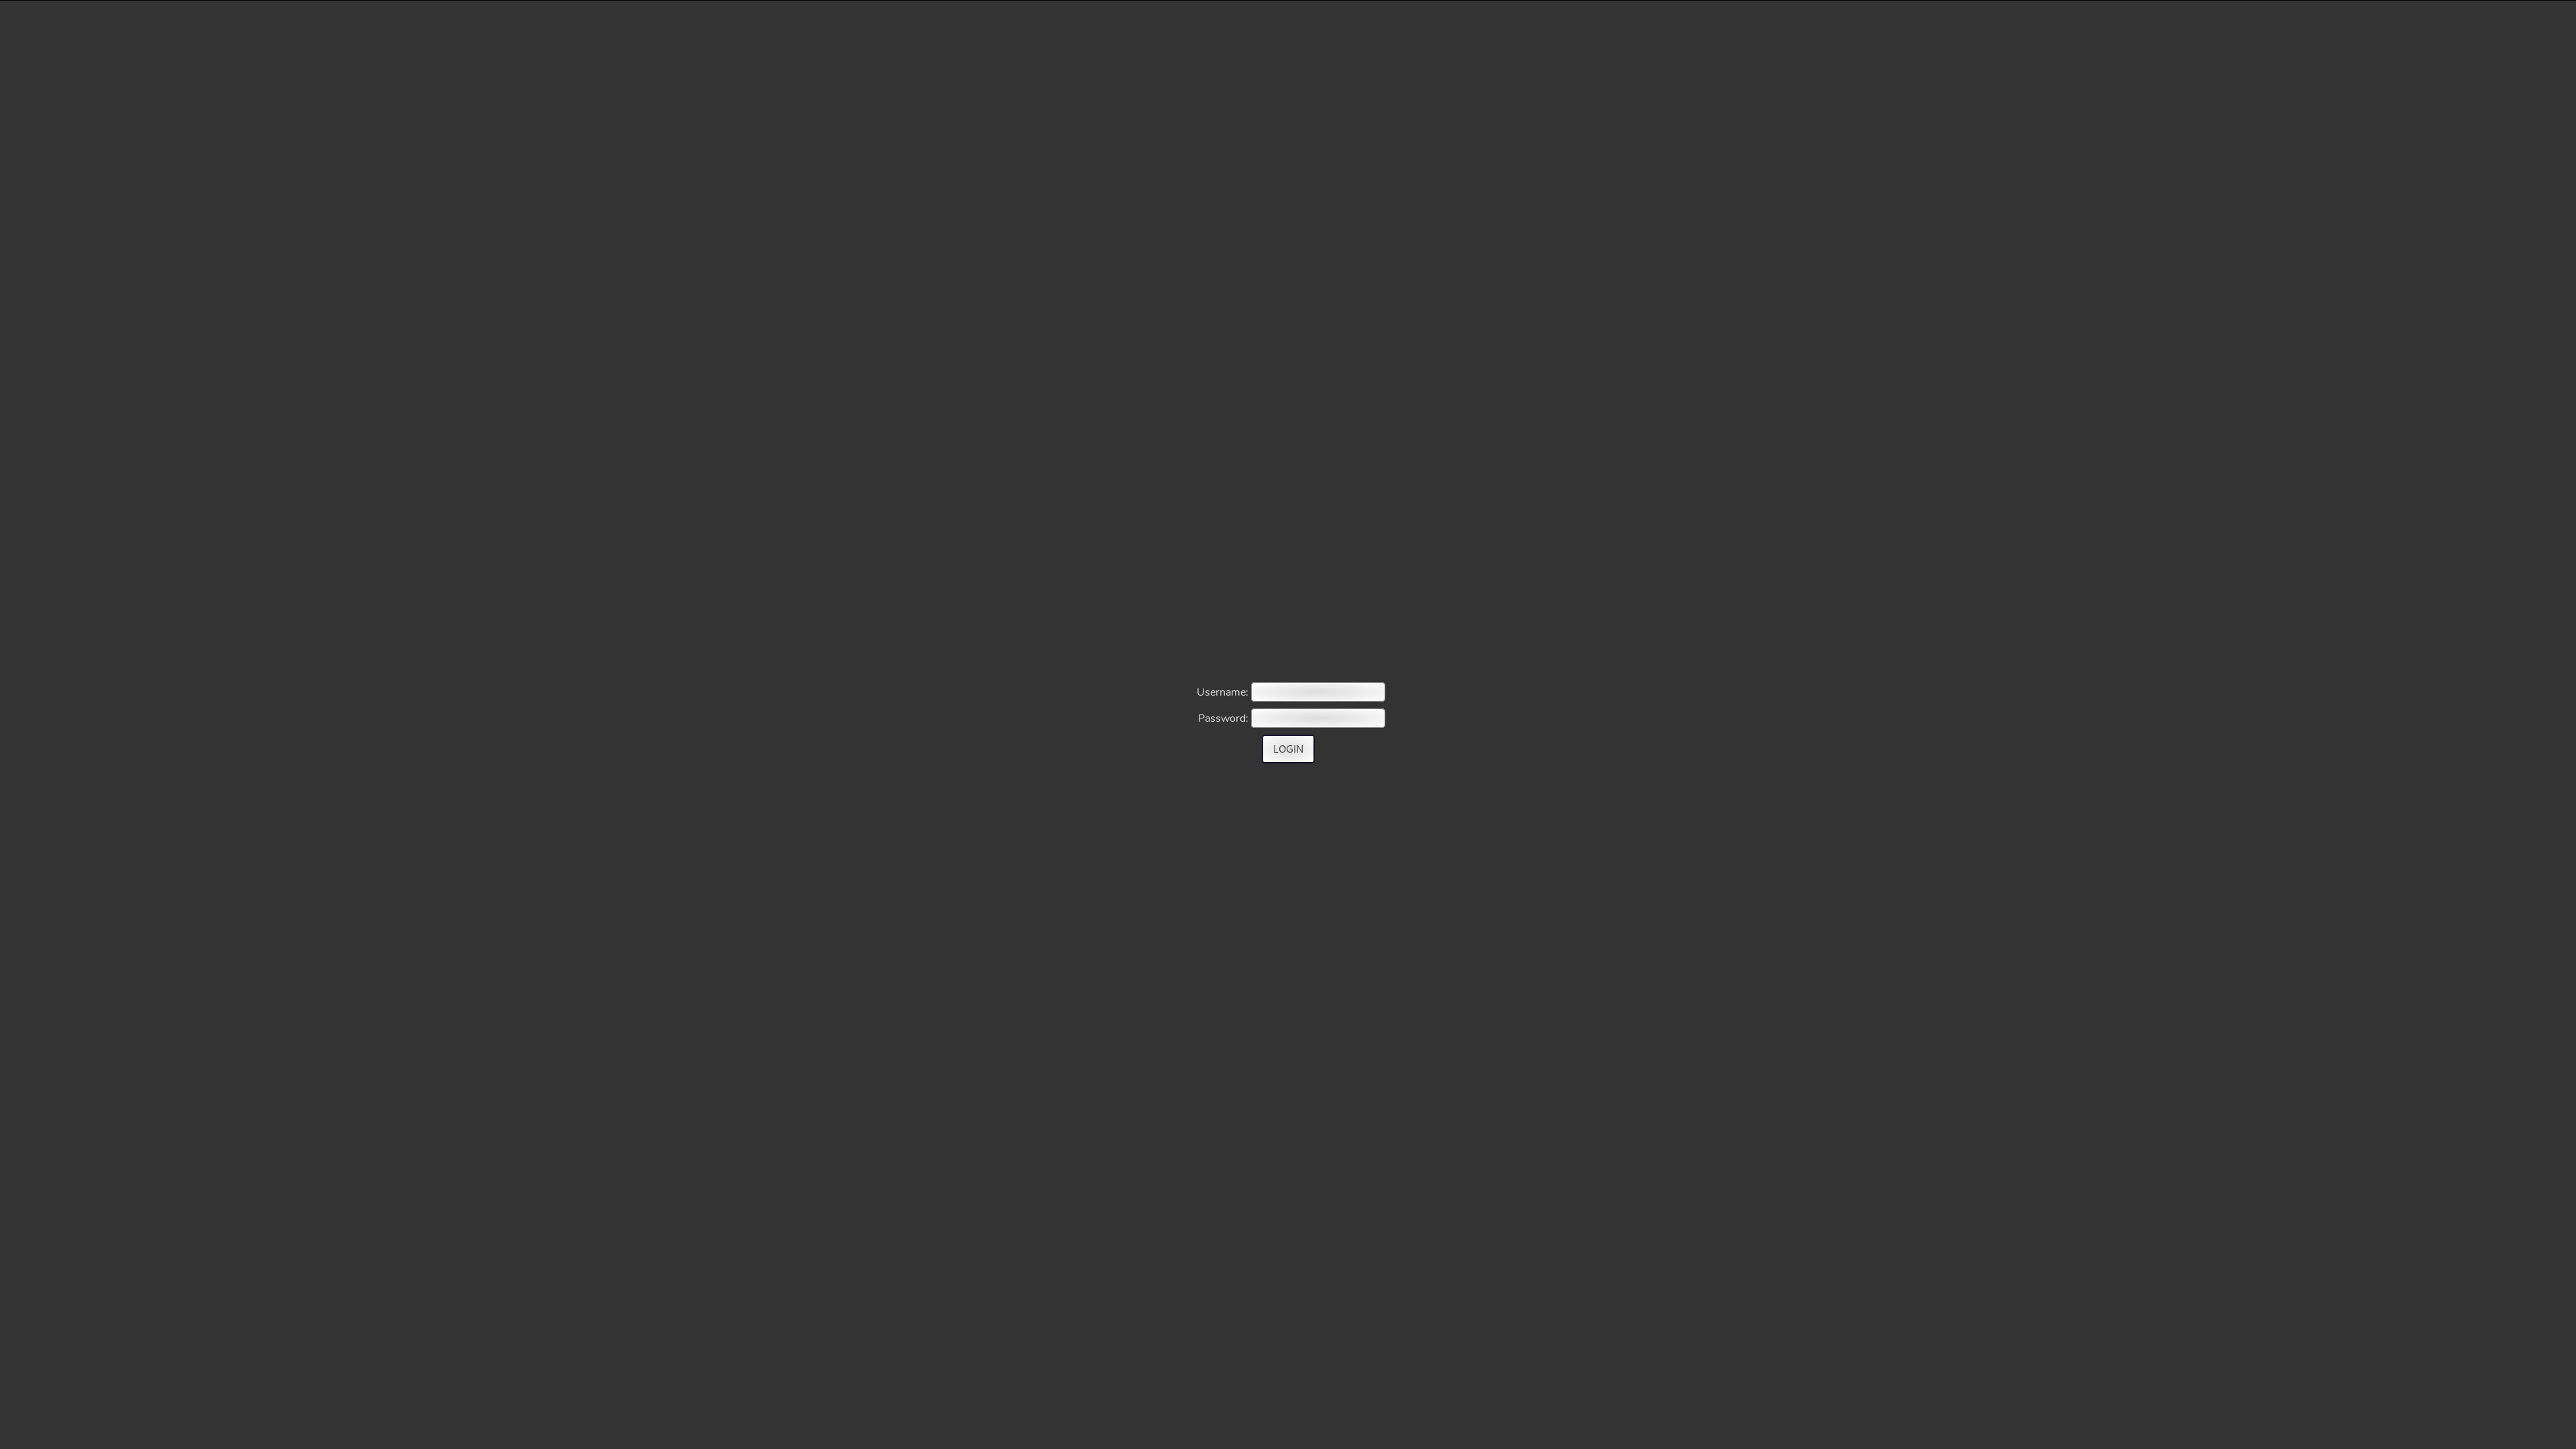
\includegraphics[width=170mm]{img/index.png}
		\caption{index.php \label{index.php}}
	\end{figure}	
	The index page has a simple layout, its just a small form for the username and password and a login button. The form always appears in the centre of the screen horizontally and vertically. If the user incorrectly logs in an error message appears in red as can be seen in Figure \ref{indexerror.php}.
	\begin{figure}[H]
		\centering
		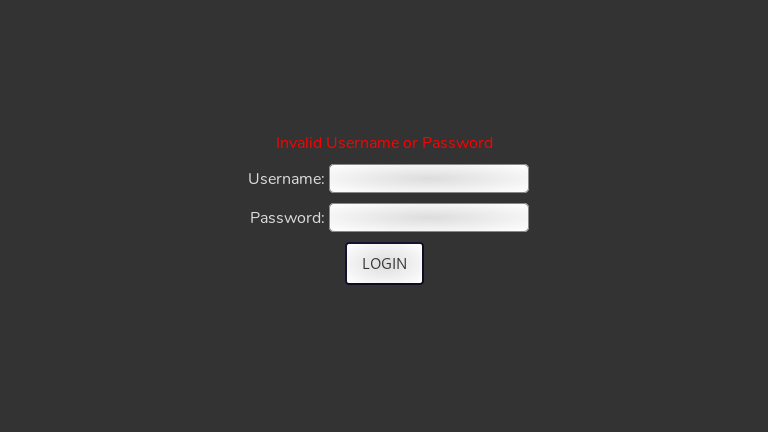
\includegraphics[width=70mm]{img/indexerror.png}
		\caption{index.php error message \label{indexerror.php}}
	\end{figure}
	The dark background with the lighter boxes brings the users attention to the form making it clear and easy to see what to do.
	\subsection{Stock}
	\begin{figure}[!ht]
		\centering
		\hspace*{-1in}
		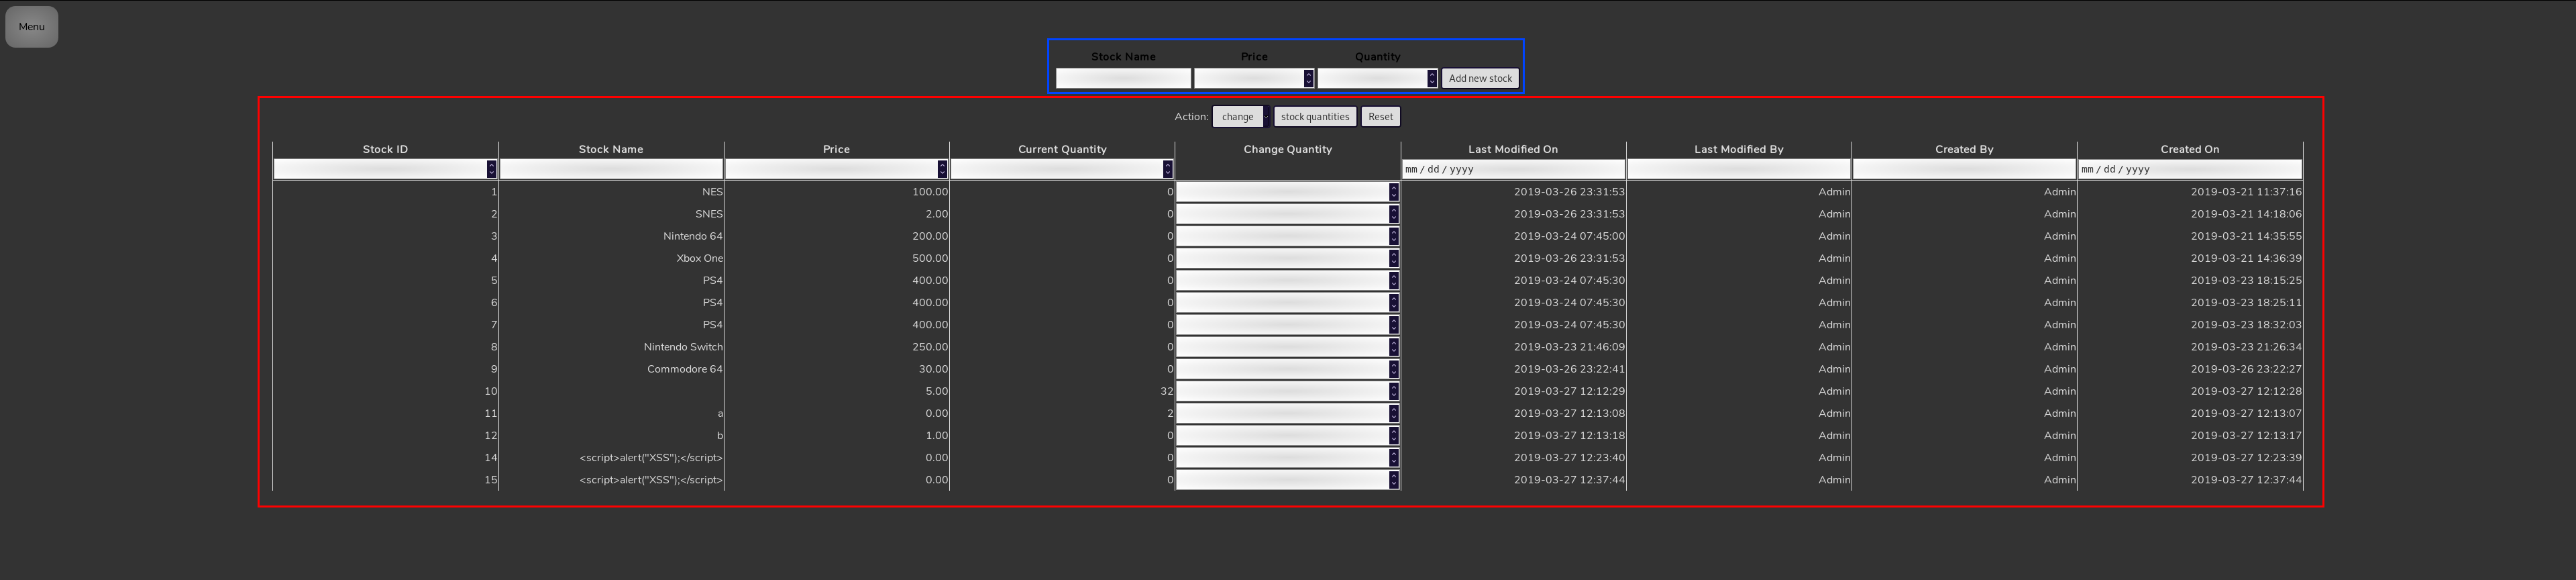
\includegraphics[width=170mm]{img/stock.png}
		\caption{stock.php \label{stock.php}}
	\end{figure}
	The stock page as seen in Figure \ref{stock.php} has three main components, the add stock form (shown in red), the change stock form (shown in blue), and the sidebar (not shown). The add stock form and the change stock form both have permission requirements to see or send. This means that if a logged in user does not have the adequate privileges the forms will form be produced by the php. There is also a check on each of the post request handlers to see if the user have permission to make the request. A session token is also generated for these forms to stop Cross Site Request Forgery. Care is also taken to stop Cross Site Scripting, you can see in the Figure that there are some attempts at XSS in the name column but these have been correctly rendered and the XSS didn't work. Like the index page the darker background highlights the forms allowing a user to see where they should put in any input. The lone button in the corner is for opening sidebar. The dark minimalist layout makes the website match the trend in design leading to modern feel. The table has three components, in descending order: the submit options, the search terms, and the quantity form. The submit options allow a user to submit their changes as "change" or "set" requests, it also allows the user to reset all the fields in the table. The search terms allow a user to filter the table to only include the results they want, this makes a request to getStock.php which in turn returns a table. The quantity form allows the user to set the quantities they want to change. Only the fields with values will be sent so the post request is smaller and takes less time to process. The sidebar on this page does not have a link to the admin page if the user does not have the correct privileges for it.
	\subsection{Admin}
	\begin{figure}[!ht]
		\hspace*{-1in}
		\centering
		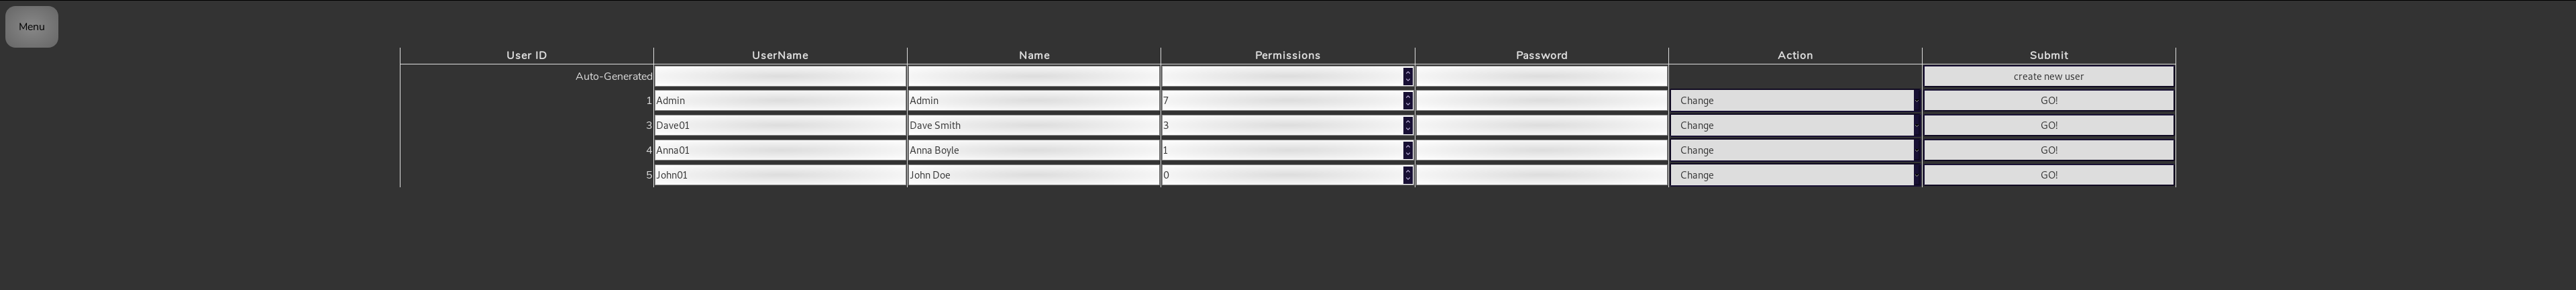
\includegraphics[width=170mm]{img/admin.png}
		\caption{admin.php \label{admin.php}}
	\end{figure}
	The admin page is only accessible to users who have admin privileges, if they do not they are redirected to the stock page. The page has a table which allows an admin to manage user accounts. The admin can add an account with with the first row and change any of the user's name, username, permissions and password. The password is hashed using bcrypt allowing it to be stored in one column of data in the database. The admin can also remove any account by changing the action field. This page allows for quick creation of new accounts for new employees or removal of accounts if they become compromised. Again this page fits with the theme with a dark background and light form inputs to bring attention to where the user can make changes. This look keeps within the modern and simple feel of the site. The sidebar, like on the stock page, is hidden until the menu button is clicked at which it appears on the right hand side.
	\newpage
	\section{Security}
	\paragraph{Cross site request forgery}
	Cross site request forgery (CSRF) is a form of attack that allows an attacker to perform action for the victim without their knowledge. A common mitigation for this is to generate a token when the logs in. This token is then inserted into all requests that the user makes. The token is checked against the one stored on the server and the request is only allowed if the tokens match. I have implemented this on all my forms that change data on the server so CSRF is not possible. Unfortunately, all CSRF protections are pointless if a the site is vulnerable to Cross site scripting.
	\paragraph{Cross site scripting}
	Cross site scripting (XSS) can be thought of as a more powerful version of CSRF, where CSRF can only make a user unknowingly perform a predefined action, XSS allows an attacker to execute arbitrary commands on the victim giving them no limit on what they can do. To protect against XSS, any place where users can input data must be sanitized and escaped properly. In PHP this can be dane with the $htmlspecialchars$ function.
	\paragraph{Password storage}
	One of the most popular words of wisdom when it comes to anything security related is: ``don't attempt to make your own encryption, other people have already done it better". This lead me to using bcrypt, which is easy to use in PHP. The $password\_hash$ function has an option for bcrypt making it an simple as changing a variable. the hashes (which also contain a salt) can be stored in a 60 byte string and verified with $password\_verify$.
\end{document}